\chapter{Méthodes}

Nous avons utilisé la base de données présentée dans la partie~\ref{lab:bdd} pour évaluer les performances des techniques de correction du mouvement respiratoire présentées dans le chapitre \ref{lab:corrMvt}. 

Les techniques de correction du mouvement implémentées sont les suivantes :

\begin{enumerate}
 \item Correction pendant la reconstruction par modification de la matrice système (voir section \ref{lab:corrMatSyst}). Elle sera désignée par l'acronyme \emph{TE-MS} (Transformation \'Elastique de la Matrice Système)
 \item Correction post-reconstruction par recalage des images prises à différents instants du cycle (voir section \ref{lab:corrPostRecon}). Elle sera désignée par l'acronyme \emph{TE-IM} (Transformation \'Elastique des Images reconstruites) 
\end{enumerate}

Elles sont comparées dans cette partie avec les images non corrigées \textbf{TE-MS} et des images statiques (qui représentent une correction parfaite). Leur acronymes sont respectivement \emph{NoCorr} et \emph{Statique}

L'objectif est d'évaluer les performances des techniques de correction du mouvement sur la détection des lésions de faible contraste et faible diamètre. Pour cela, les performances d'un système de détection automatique seront mesurées à l'aide des courbes F-ROC.

La suite de ce chapitre présente les caractéristiques principales du système d'aide à la détection (CAD) que nous avons utilisé (voir chapitre \ref{lab:chapCAD}), l'étape d'optimisation du CAD que nous avons utilisé, puis la méthode utilisée pour mesurer les performances de détection.

\section{Système CAD} % 11.1

Le système CAD que nous utilisons a été développé à l'origine pendant les travaux de thèse de Sandrine Tomeï ainsi que mes travaux de master~\cite{tomei2008automatic,lartizien2010impact}. Nous l'avons amélioré et adapté aux besoins de cette étude, notamment en développant les mesures de performances.


Le CAD utilise des informations fréquentielles obtenues par décomposition des images en ondelettes biorthogonale 4/4 non décimée (figure \ref{fig:ondelettes}) . Ces données sont utilisées par le système de classification basé sur un SVM travaillant voxel par voxel. Une étape de réduction des faux positifs est ajoutée par la suite.

Le nombre de tumeurs utilisées pour générer la base d'apprentissage est de 107 pour la base d'apprentissage poumon et 173 pour la base d'apprentissage foie. Ce nombre est relativement faible~\cite{hua2005optimal} par rapport à la taille du vecteur de caractéristiques utilisé pour le CAD (entre 24 et 32), ce qui nécéssite de prendre en compte un maximum de données pour l'apprentissage et le test pour éviter le sous-apprentissage. Nous avons donc utilisé une méthode d'évaluation des performances par resubstitution. Cela signifie que les apprentissages et les tests sont réalisés sur la même base de données constituée de 15 patients présentés dans le chapitre \todo{vérifier} 5. %\ref{lab:bdd}.

\subsection{Vecteur de Caractéristiques}

Nous avons choisi d’utiliser une décomposition en ondelettes 3D non décimées par banc de filtres. Dans le cas tridimensionnel, la décomposition par banc de filtres est résumée par la figure \ref{fig:ondelettes}. L’image de départ est traitée successivement dans les trois directions de l’espace par un filtre fréquentiel passe-haut correspondant à la fonction d’ondelettes (noté $H$) et passe-bas correspondant à la fonction d’échelle (noté $L$). 

\begin{figure}
 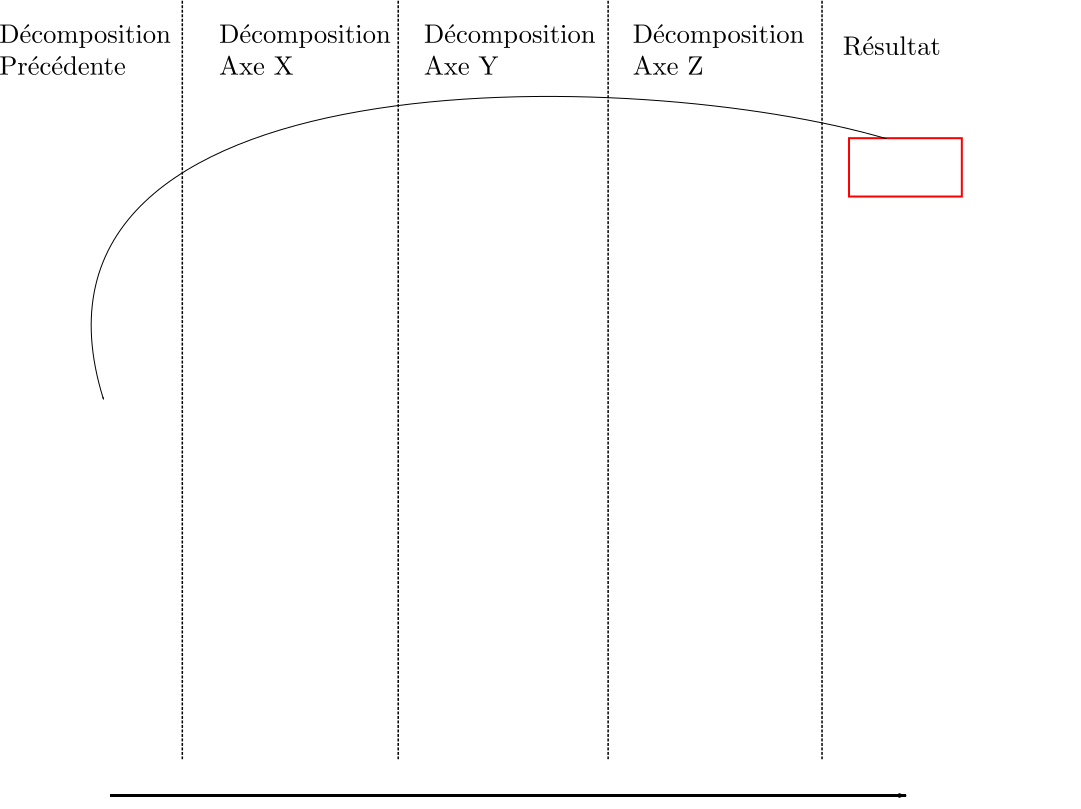
\includegraphics[width=15cm]{images/decompHotell}
 \caption[Décomposition en ondelettes par banc de filtres]{Décomposition en ondelettes par banc de filtres : Chaque image est filtrée selon les 3 dimensions pour obtenir les coefficients d'ondelettes et d'échelle de chaque voxel de l'image. L correspond à un filtrage passe-bas tandis que H corresponds à un filtrage passe-haut. Les coefficients d'échelle sont contenus dans l'image $LLL_{j+1}$ tandis que les coefficients d'ondelettes sont présents dans les sept images de détail $LLH_{j+1}$, $LHL_{j+1}$ \dots $HHH_{j+1}$ }
 \label{fig:ondelettes}
\end{figure}

\begin{figure}
 \centering
 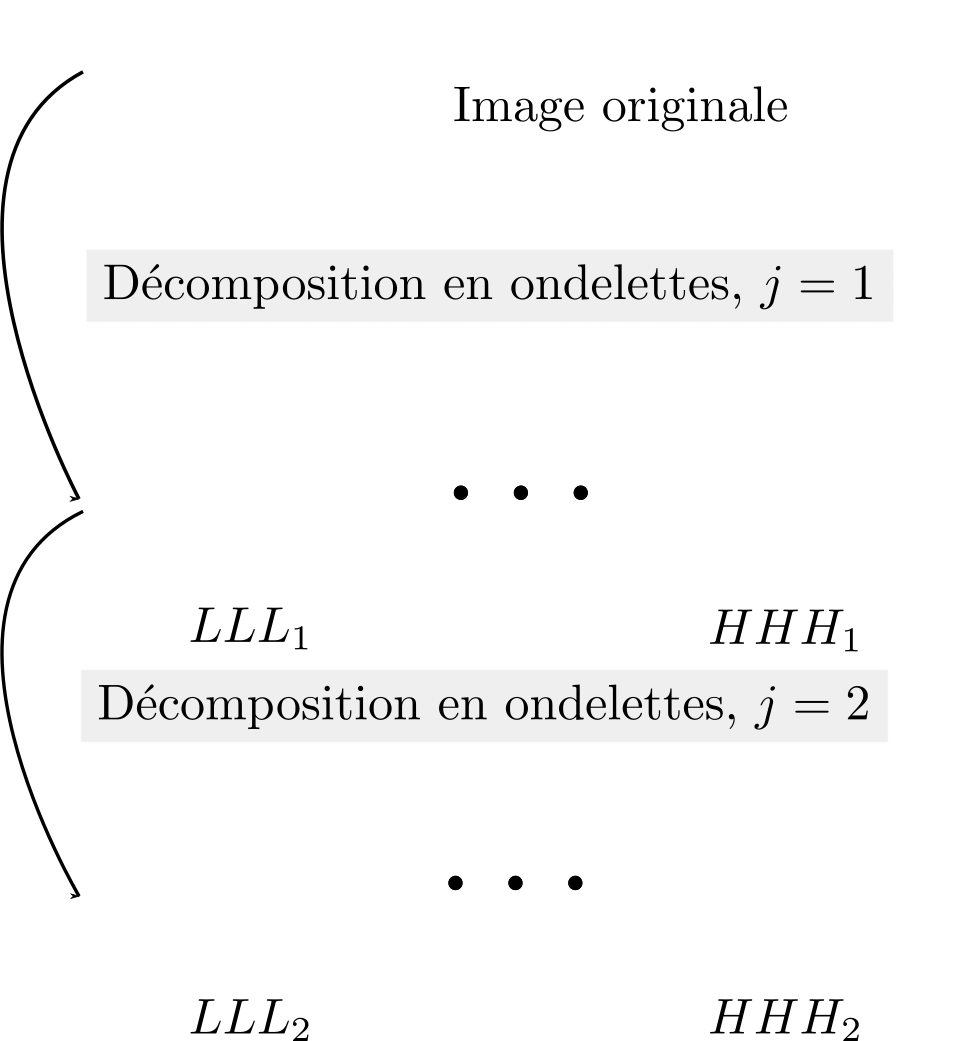
\includegraphics[width=15cm]{images/exemplesDecomp}
 \caption[Exemples de décomposition d'images en ondelettes]{Exemples d'images TEP décomposées en ondelettes. Sont représentées l'image originale, puis l'image des coefficients d'échelle notée $LLL_j$ et une image des coefficients d'ondelettes notée $HHH_j$ pour deux niveaux de décomposition. L'ondelette utilisée pour la décomposition est la biorthogonale 4/4}
 \label{fig:bior44Ex}
\end{figure}


Ainsi sept images de détails (HHH, LLH, \dots) et une image d’approximation (LLL) sont produites pour chaque niveau $j$ de décomposition. Les huit images du niveau suivant $j+1$ sont générées de la même manière, mais en considérant l’image d’approximation $LLL_j$ du niveau précédent comme image de départ. Les caractéristiques des images, rassemblées dans un vecteur descripteur de taille $8 \times j$, correspondent ici à l’ensemble de ces coefficients pour chaque voxel  de l’image. Des exemples d'images obtenues par les filtrages sont présentés dans la figfure \ref{fig:bior44Ex}.

Nous utilisons l'ondelette biorthogonale 4/4 dont la fonction est présentée sur la figure \ref{fig:bior44}.


\begin{figure}
 \begin{tabular}{ c c }
 
 \includegraphics[width=8cm]{images/bior44Ondelette} & \includegraphics[width=8cm]{images/bior44Echelle} \\
 Fonction d'ondelette & Fonction D'échelle\\
 \end{tabular}

 \caption{Fonction d'ondelette et d'échelle biorthogonale 4/4}
 \label{fig:bior44}
\end{figure}

\subsection{Génération de la base d'apprentissage}
Les données générées par la décomposition en ondelettes de chaque image se présentent sous la forme de volumes 4D, indiquant pour chaque voxel de l'image 3D l'ensemble des $8 \times j$ coefficients associés.

La base d'apprentissage sert à entraîner le classifieur dans un processus de classification supervisée, en lui fournissant un ensemble d'exemples avec leur classes associées (voir figure \ref{fig:fonctClassif}) page \pageref{fig:fonctClassif}).

La génération de cette base demande l'extraction de points de la classe ``pathologique'', et de la classe ``sain''. Pour chaque tumeur de la vérité terrain, nous extrayons de l'image correspndante le vecteur de caractéristiques du voxel placée au centre de la tumeur. Ce vecteur de caractéristique correspond aux coefficients de la décomposition en ondelette du voxel de l'image ($8 \times j$).

Les points de la classe ``sain'' sont extraits de manière aléatoire dans les volumes de toutes les images (hors tumeurs). Pour des raisons de simplicité d'implémentation, un nombre fixe de points est extrait de chaque image.

\subsection{Apprentissage de la Machine à Vecteur de Support (SVM)}

La base de données d'apprentissage est utilisée  par le classifieur SVM (Machine à Vecteur de Support) pour l'apprentissage.

Le principe des SVM est de trouver l’hyperplan optimal de séparation dans l'espace des caractéristiques, qui va maximiser la marge de séparation entre les deux classes ``pathologique''  et ``sain'' (le SVM est défini plus en détail en \ref{lab:SVM}). Cette marge correspond à la distance entre les plus proches vecteurs de caractéristiques appartenant à chacune des classes et l'hyperplan. La définition de cette marge et donc de l’hyperplan, se fait uniquement à partir de vecteurs de support, qui correspondent à l'enveloppe du groupement de point de chacune des deux classes.

Le SVM va calculer un modèle décrivant l'hyperplan permettant de séparer les données.

\subsection{Génération des sites présumés}
\label{lab:aggregatsCAD}
Une fois le classifieur entraîné, il est capable de classer rapidement les nouveaux vecteurs de caractéristiques. Ainsi, on lui soumet les données correcpondants aux voxels des images pour qu'il les classe. On obtient donc en sortie un ensemble de cartes de score (une par image 3D), dans lesquelles chaque voxel correspond au score indiqué par le SVM. Ce score est une mesure de distance polarisé par rapport à l'hyperplan de séparation dans l'espace des points d'apprentissage, et donne en plus de la classe, donc une mesure de la ``certitude'' du SVM vis-à-vis de sa classification.

Cette carte de score est ensuite seuillée pour fournir une carte binaire, indiquant pour chaque voxel la classe sélectionnée par le SVM pour ce niveau de seuil. Le mécanisme de sélection du seuil est défini en \ref{lab:selectionSeuil}. Une exemple de carte de score est visible dans la figure \ref{fig:cheminementCAD}.a.
	
\`A cette étape, le résultat est sous forme d'une carte de voxels étiquetés comme ''sain`` ou ''pathologiques``. Nous avons choisi de travailler sur des agrégats de points plutôt que directement sur les voxels car les cartes binarisées sont relativement bruitées (voir \ref{fig:cheminementCAD}.b), et donc non directement exploitables. Les voxels ``pathologiques'' sont donc regroupés selon une 26-connexité (3x3x3). Un score est associé à chaque  agrégat, correspondant au score le plus important observé dans l'agrégat.

\subsection{Règles d'évaluation du résultat}
\label{lab:reglesSelect}
Pour évaluer le résultat, nous avons élaboré des règles permettant de classer les agrégats à l'aide de la vérité terrain. Ce sont ces algorithmes qui sont utilisés dans les évaluateurs de performances présentés ci-après.

Les agrégats sont classés en LL (Lésion localisée) et NL (Non Lésion) selon qu'ils peuvent être considérés comme des vrais positifs ou des faux positifs :

Soit $\mathbf{L}$ l'ensemble des points de la lésion, $\mathbf{A}$ les points correspondant à l'amas candidat.

Les agrégats seront considérés comme des vrai positifs si ils intersectent une tumeur selon les règles décrites ci-après, ou comme de faux positifs dans le cas contraire. Cependant, si leur taille est inférieure à la taille minimale définie par la première règle, l'amas n'est pas considéré.

Règles de classification :
\begin{enumerate}
 \item $card( \mathbf{L} \cap \mathbf{A} ) > \alpha \times card( \mathbf{L} )$ : où $\alpha$ qui définie la proportion minimale de la tumeur qui doit être présente dans l'amas. Elle permet d'éviter les amas qui intersecteraient la tumeur par accident.
 \item $card( \mathbf{L} \cap \mathbf{A} ) > \beta \times card( \mathbf{A} )$ : où $\beta$ qui limite l'étendue de l'amas en dehors de la tumeur.
\end{enumerate}

$\alpha$ et $\beta$ sont des constantes empiriques fixées respectivement à 0.05 et 0.20 dans nos travaux. Nous avons choisit ces valeurs en visualisant les cartes de score pour obtenir des résultats correctes sans pénaliser les performances.

\subsection{Résumé}

Ce pseudo-code décrit les différentes étapes du CAD, depuis l'importation des images jusqu'à à l'extraction des lésions potentielles. Il est illustré par la figure \ref{fig:cheminementCAD} :

\begin{figure}
 \centering
 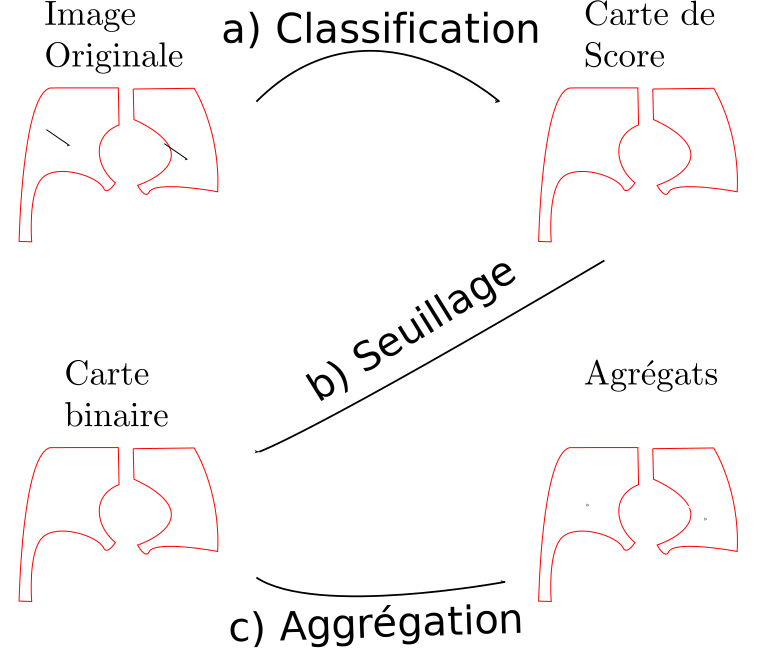
\includegraphics[width=15cm]{images/cheminementCAD}
 \caption{Schéma du système CAD : l'image d'origine en haut à gauche est utilisée par le classifieur pour générer la carte de score. Cette carte est ensuite seuillée par l'étape b) pour générer une carte binaire correspondant aux sites qui dépassent un certain score $s$. L'étape c) correspond à la formation des agrégats qui seront le résultat du système CAD. Cette étape s'accompagne d'une suppression des sites de trop petite taille. Les flèches représentent des lésions dans l'image d'origine}
 \label{fig:cheminementCAD}
\end{figure}

\begin{enumerate}
 \item Décomposition des images en ondelettes : pour chaque voxel de l'image d'origine, on obtient entre 8 et 32 coefficients suivant le niveau de décomposition de l'image, qui correspondent au vecteur de caractéristiques utilisé par le classifieur.
 \item Extraction de la base d'apprentissage : les coefficients des centres de toutes les tumeurs sont extraits des volumes décomposés, et vont former la base d'apprentissage pathologique. Un certain nombre de voxels sont tirés aléatoirement dans les zones normales de chaque image et leurs coefficients sont ajoutés à la base saine.
 \item Apprentissage : le classifieur SVM est entraîné sur cette base d'apprentissage pour générer le modèle qui sera utilisé pour le test.
 \item Tests : le SVM entraîné est utilisé pour classer chaque voxel contenu dans les organes à évaluer (poumon et foie).
 \item Réduction des faux-positifs : les points sont agrégés en composantes connexes (26-connexité en 3 dimensions).
 \item Évaluation : lorsque nous avons accès à la vérité terrain, il est possible d'évaluer les performances du CAD en classant les agrégats en LL (Lésion Localisée) et LN (Lésion Non Localisée).
\end{enumerate}



\section{Optimisation des paramètres du système CAD} % 11.2
\label{lab:optim}

Les différentes étapes de l'évaluation des performances nécessitent de fixer un grand nombre de paramètres que nous allons détailler dans cette partie.

\subsection{Paramètres à optimiser} % 11.2.1


\subsubsection{Paramètres de la base d'apprentissage}

Nous avons sélectionné plusieurs paramètres qui, selon nous, peuvent influencer les performances de détection. Ces paramètres sont assez généraux et seront donc sélectionnés une fois et appliqués à tous les jeux de données de la même manière :

\begin{description}
 \item[Normalisation :] les données sont normalisées de deux manière différentes : modifier les données pour que la moyenne et l'écartt-type aient une valeur respectivement de 0 et 1 ($(\mu, \sigma)=(0,1)$) noté \emph{moyenne}, ou alors le adapter pour que l'ensemble des valeurs soit comprises entre -1 et +1, noté \emph{écart}.
 \item[Nombre de points de la base d'apprentissage :] Le nombre de points extraits de chaque image pour alimenter la base d'exemples normaux peut avoir une influence sur les résultats. Nous avons testé trois valeurs. 100 points par images (pts/im.) (soit 1500 pts. négatifs), 200 pts/im. (soit 3000 pts. négatifs) et 1000 pts/im. (soit 15000 pts. négatifs).
 \item[positions des points extraits :] Les points normaux extraits de la base d'images peuvent être extraits de tout le volume de l'organe hors tumeurs, ou bien extraits sur une sous-partie seulement de l'organe en éliminant les bords de l'objet une érosion morphologique de rayon deux voxels.
\end{description}

Le but de la normalisation est d'homogénéiser les plages de valeurs des différentes caractéristiques pour faciliter le travail du classifieur, dont les paramètres $C$ et $\gamma$ (définis ci-après) dépendent de la distance entre les points et ne permettent pas de gérer des différences trop importantes d'étendues dans les caractéristiques. La première méthode de normalisation (\emph{moyenne}) a l'avantage d'être relativement peu sensible aux valeurs extrêmes, contrairement à la seconde (\emph{écart}).

Le nombre de point de la base d'apprentissage détermine directement la qualité de l'apprentissage. Le nombre de caractéristiques est de $8 \times j$, avec $j$ le niveau de décomposition des images. Il n'existe pas de règle définitive pour choisir le nombre d'exemples nécessaires en fonction du nombre de caractéristiques, mais les SVM sont relativement efficaces à éviter le sur-apprentissage. Dans notre cas, il serait donc préférable d'avoir plus de données. Cependant, le nombre de points notés ``tumeurs'' est limité par le nombre de tumeurs présentes dans la base d'apprentissage (173 tumeurs pour le poumon, 106 pour le foie). Il y a donc un risque de déséquilibre de la base d'apprentissage, qui devrait idéalement avoir le même nombre d'exemples ``pathologique'' que ``sain``. Il est possible de corriger ces déséquilibres en indiquant un paramètre C différent pour chaque classe, mais les tests que nous avons réalisés ne montrent aucun changement dans les résultats.

Les points normaux extraits des images pour alimenter la base vont avoir une influence directe sur la qualité des résultats. Idéalement ils devraient être représentatifs de l'ensemble des cas rencontrés dans la base de tests, néanmoins les bords de certains organes ont un profil proche de celui des tumeurs, et rendent l'estimation de la surface de séparation plus difficile. Nous avons donc voulu évaluer la performance du CAD sur une base dépourvue de ces données ambiguës. Pour cela nous avons réalisé une érosion de 2 voxels sur les masques des volumes sains à extraire.

\subsubsection{Paramètres du classifieur}
\label{lab:paramClassif}
Le classifieur (SVM) utilise en entrée les données d'apprentissage formatées selon les choix opérés précédemment (normalisation, volumes utilisés pour extraire les points de la base de points ''sain`` et nombre de ces points) et va générer un modèle. Cependant, cet algorithme dispose de ses propres paramètres, qui sont beaucoup plus dépendant des données (voir \ref{lab:SVM}). Un nouveau jeu de paramètres sera donc calculé pour chaque type de correction du mouvement respiratoire.

\begin{description}
 \item[Niveau de décomposition $j$ :] il correspond au nombre de niveaux de décomposition pris en compte par le SVM. Les niveaux de décomposition élevés correspondant à des informations de très basse fréquence, les informations qu'ils apportent ne sont pas forcément pertinentes pour la détection des lésions. Cependant, les caractéristiques fréquentielles des images générées par les différents jeux d'images étant différentes, il est nécessaire d'adapter ce paramètre pour chaque niveau.
 \item[Coefficient de pénalisation $C$ :] lors du calcul de l'hyperplan de séparation des données, chaque point mal classé va pénaliser la surface selon un facteur proportionnel à $C$.
 \item[Largeur de bande $\gamma$ :] cette valeur influe directement sur la largeur de bande du noyau utilisé par le classifieur (Fonction de Base Radiale gaussienne, ou RBF).
\end{description}

\subsection{Méthodes d'optimisation}

La sélection du triplet de paramètres $(C, \gamma, j)$ vu précédemment est obtenue à l'aide des algorithmes présentés ci-après. 

\subsubsection{Choix des paramètres du classifieur}

Pour obtenir les meilleurs paramètres du classifieur, nous réalisons une recherche exhaustive par grille. Cela correspond à évaluer les performances sur le produit cartésien d'une discrétisation des valeurs de chaque paramètre.

Par exemple, si nous disposons de deux paramètres A et B, et que nous recherchons le meilleur jeu de paramètres, il faut tout d'abord sélectionner pour chaque paramètre la taille de la zone de recherche. Pour A, ce sera les valeurs {-1, 0, 1, 2} et pour B les valeurs {100, 10000, 50000}. Les critères de performance seront évalués pour toutes les combinaisons des valeurs de A et B, tels que (-1, 100), (-1, 10000), (-1, 50000), (0, 100), \dots, (2, 50000). Le jeu de paramètres ayant obtenu les meilleures performances sera donc sélectionné. 

Les critères de performance que nous avons sélectionnés sont la sensibilité et la spécificité obtenue pour une validation croisée à 5 éléments réalisée sur la base d'apprentissage comme présenté sur la figure \ref{fig:crossValid}. La validation croisée permet de réduire le biais sur les performances~\cite{varma2006bias}.

\begin{figure}[h!]
 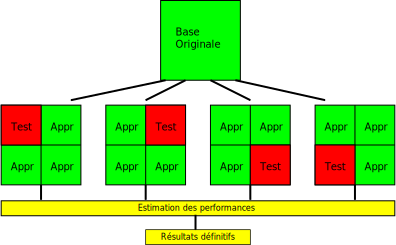
\includegraphics[width=15cm]{images/crossValid}
 \caption{Réalisation d'une validation croisée à $n$ éléments (ici 4) : La base d'exemples d'origine est décomposée en $n$ parts égales. La mesure de performance se fait $n$ fois, avec à chaque fois un apprentissage sur $n-1$ éléments et un test sur l'élément restant. La mesure de performance est réalisée sur les résultats des $n$ tests.}
 \label{fig:crossValid}
\end{figure}


Pour choisir les meilleurs paramètres du classifieur, j'ai effectué une recherche exhaustive par grille avec les paramètres suivants :

\begin{description}
 \item [$C$ :] de 1 à 10000 en 15 pas logarithmiques
 \item [$\gamma$ :] de 0.0001 à 1 en 15 pas logarithmiques
 \item [$j$ :] de 1 à 4, soit de 8 à 32 caractéristiques
\end{description}

L'optimisation a été réalisée à l'aide du logiciel rapid-i~\cite{mierswa2006} pour chaque type d'image. Les indicateurs de performance calculés par validation croisée sont les suivants : sensibilité, spécificité et précision dafinis en \ref{lab:pressensib}. Le triplet de paramètres retenu est celui qui maximise la sensibilité.

Nous avons représenté pour chaque jeu d'image le nuage de points correspondant à la répartition de chaque triplet ($C, \gamma, j)$ dans un espace à deux dimensions (``Sensibilité'', ``Spécificité''). Cela permet de vérifier que le critère choisi (maximisation de la sensibilité) ne se fait pas trop au détriment de la spécificité.

De ce nuage de point nous pouvons voir le front de Pareto. Ce type de diagramme permet de rechercher un optimum selon plusieurs critères antagonistes. Dans notre cas, nous voulons à la fois une sensibilité et une spécificité importante, sachant qu'il n'existe pas de jeu de paramètres ''parfaits`` qui permettent d'avoir 100\% aux deux. Dans notre cas, le front de Pareto va permettre de vérifier que le choix par maximisation de la sensibilité ne se fait pas au détriment de la spécificité.


\subsection{Mesure de performance de détection}
\label{lab:selectionSeuil}
La mesure de performances décrite ici permet de sélectionner les meilleurs paramètres de génération de la base d'apprentissage, mais aussi une fois ces paramètres sélectionnés, de comparer les différentes techniques de correction du mouvement respiratoire. La recherche des meilleurs paramètres de la base d'apprentissage sera réalisée sur la base d'images statiques afin de ne pas être influencée par les éventuels artefacts des autres type d'images.

Pour un seuil donné, Le CAD va générer un ensemble d'agrégats associés à un score, comme présenté en \ref{lab:aggregatsCAD}. Il est ensuite possible d'évaluer la performance de ce CAD à l'aide de courbes F-ROC décrites en \ref{lab:FROC} construites à l'aide de la vérité terrain.

Le seuil sélectionné $s$ pour générer les agrégats est celui qui maximise la Fraction de Localisation de Lésion (FLL), c'est à dire celui qui va permettre de détecter un maximum de lésions. 

Cette sélection est réalisée selon l'algorithme suivant :

Le processus d'estimation de la sensibilité pour un seuil $s$ se fait de la manière suivante : Tout d'abord les cartes de scores sont binarisées en fonction de $s$. Les agrégats sont estimés sur ces cartes binaires, en prenant en compte les informations provenant des cartes de score correspondantes pour attribuer un score à chaque agrégat. Ils sont ensuite classés en ''Lésion localisée`` (LL) ou ''Non Lésions`` (NL) à l'aide de la vérité terrain, selon les règles présentées en \ref{lab:reglesSelect}. Une valeur de sensibilité est calculée à partir de ces informations pour le seuil $s$.

Le seuil optimal retenu est celui qui maximise la sensibilité. Nous recherchons ce maximum pour 40 valeurs réparties de manière uniforme entre -2 et +2. Nous utilisons une recherche exhaustive car le résultat possède de nombreux minimums locaux et le temps de calcul est faible (moins d'une heure pour les 40 valeurs).

Ce critère de sélection va naturellement engendrer un grand nombre de faux positifs, mais il faut garder à l'esprit qu'il sera utilisé pour réaliser des courbes F-ROC, qui indiquent une spécificité pour chaque nombre de faux positif en jouant sur un second seuil, toujours supérieur à celui retenu pour extraire les agrégats.

Le second critère utilisé pour comparer les bases d'apprentissage est la figure de mérite décrite en \ref{lab:AFROC}. Elle va comparer pour chaque image le score du faux positif le plus haut avec les score des vrais positifs de l'image.


\chapter{Analyse des résultats}

Dans ce chapitre nous détaillons les résultats obtenus par les méthodes présentées précédemment. Nous commençons par présenter les courbes obtenues lors de l'étape d'optimisation et d'adaptation du CAD aux données, puis nous parlons des performances de détection obtenues par ce CAD sur les lésions hépatiques et Pulmonaires pour les différentes méthodes de correction du mouvement respiratoire.

Dans tous les cas, l'estimation des performances se fait de la manière suivante :

\begin{itemize}
 \item Optimisation des paramètres du classifieur au jeu de données.
 \item Comparaison des courbes Free-ROC.
 \item Comparaison des Figures de Mérite.
 \item Conclusion
\end{itemize}


\section{Optimisation des paramètres}

Nous avons réalisé des mesures de performances pour les différentes valeurs des paramètres suivants :

\begin{itemize}
 \item Nombre de points de la base d'apprentissage (100, \emph{200}, 1000)
 \item Normalisation des données (\emph{moyenne}, écart)
 \item Position des points de la base d'apprentissage (\emph{organe complet}, organe avec érosion)
\end{itemize}

Pour sélectionner le jeu de paramètre optimal, nous avons crée une base \textbf{Témoin} comprenant les valeurs en italique des paramètres présentés ci-dessus. Toutes les autres bases reprennent les valeurs de la base Témoin en modifiant un seul paramètre. Nous utiliseront par la suite les termes définis ci-dessous pour qualifier les 5 jeux de paramètres :

\begin{description}
 \item[Base Témoin : ] contient des données normalisées par la méthode ''moyenne`` avec 200 points sains extraits de chaque ensemble du volume des organes.
 \item[Base Érodée : ] contient des données normalisées par la méthode ''moyenne`` avec 200 points sains extraits du volume de chaque organe érodé (érosion morphologique de 2 voxels).
 \item[Base Appauvrie : ] contient des données normalisées par la méthode ''moyenne'' avec 100 points sains extraits de l'ensemble du volume de chaque organe.
 \item[Base Enrichie : ] contient des données normalisées par la méthode ''moyenne`` avec 1000 points sains extraits de l'ensemble du volume de chaque organe.
 \item[Base Normalisée \'Ecart : ] contient des données normalisées par la méthode ''écart`` avec 200 points sains extraits de l'ensemble du volume de chaque organe.
\end{description}

Pour vérifier que les résultats de la sélection des paramètres du classifieur sont stables, une seconde base témoin (\textbf{Témoin 2}) a été générée avec les données de seulement 14 images sur les 15 que nous avons simulées. Les points ''sains`` ne sont pas non plus extraits aux mêmes endroits que pour la base \textbf{Témoin}. Nous allons donc vérifier que les paramètres optimaux du CAD pour un jeu de données ne sont pas dépendants de la base.


\subsection{Sélection des meilleurs paramètres du classifieur}
\begin{figure}[h!]
\begin{center}
 \includegraphics[width=14cm]{images/pareto_param_200.png}

{\small a) Base Témoin}
\vspace{0.5cm}

\includegraphics[width=14cm]{images/pareto_param_100.png}

{\small b) Base appauvrie}

 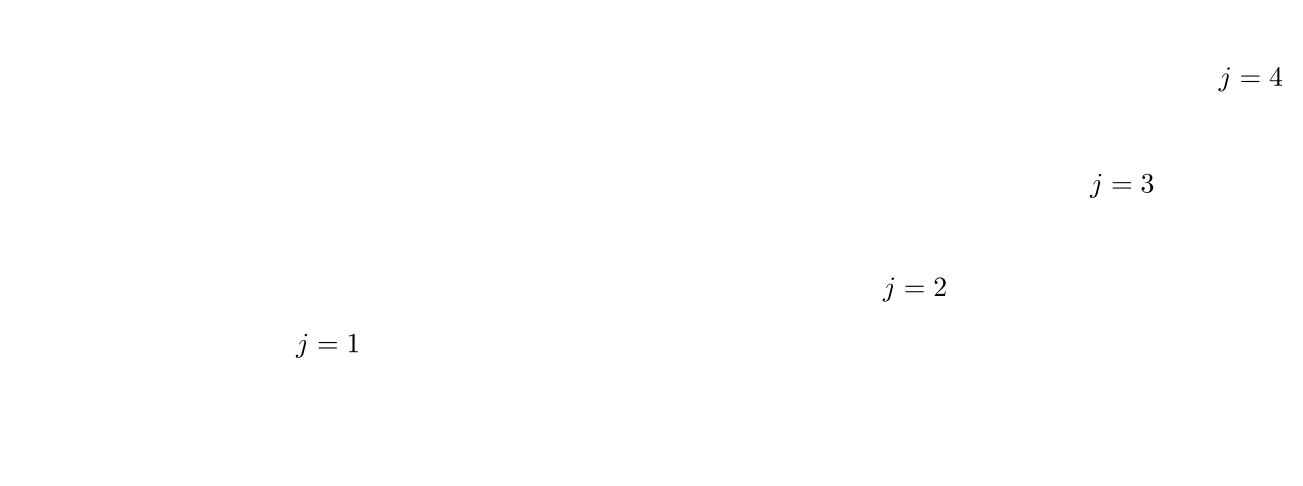
\includegraphics[width=14cm]{images/pareto_param_1000.png}
 
{\small c) Base enrichie}

\end{center}
 \caption{(1/2) Fronts de Pareto des résultats de la recherche des meilleurs paramètres du classifieur. Pour chaque triplet de paramètres $(C, \gamma, j)$, la sensibilité et la spécificité sont reportées sur le graphique. Le code de couleurs correspond à la valeur de j. Bleu corresponds à $j=1$, turquoise à $j=2$, vert à $j=3$ et rouge à $j=4$. En a), la base \textbf{Témoin}, avec 200 points négatifs par image et une normalisation \emph{moyenne}, en b) la base \textbf{Appauvrie} avec 100 points négatifs par image et une normalisation \emph{moyenne}, et en c) la base \textbf{Enrichie} avec 1000 points négatifs par image et une normalisation \emph{moyenne}.}
\label{fig:paretoParams1}
\end{figure}



\begin{figure}[h!]
\begin{center}


\includegraphics[width=14cm]{images/pareto_param_range.png}

{\small a) Base Normalisée -1/+1}

\vspace{0.5cm}

\includegraphics[width=14cm]{images/pareto_param_erosion.png}

{\small b) Base Érodée}

 \includegraphics[width=14cm]{images/pareto_param_200_2.png}

{\small c) Base Témoin 2}

\end{center}
 \caption{(2/2) Fronts de Pareto des résultats de la recherche des meilleurs paramètres du classifieur. Pour chaque triplet de paramètres $(C, \gamma, j)$, la sensibilité et la spécificité sont reportées sur le graphique. Le code couleur correspond à la valeur de j. En a) la base \textbf{Noamrlisée Écart} avec 200 points négatifs par image et de normalisation écart. En b), la base \textbf{Érodée}, avec 200 points négatifs par image et une normalisation \emph{moyenne}, en c) la base \textbf{Témoin 2}, réalisée de la même manière que la base \textbf{Témoin} mais en retirant une image. }
\label{fig:paretoParams2}
\end{figure}


Les paramètres du classifieur sont déterminés par une recherche par grille. Elle consiste à rechercher l'optimum en évaluant la performance de chaque jeu de paramètre dans un ensemble déterminé à l'avance. La performance de chaque triplet $(C, \gamma, j)$ est estimée en réalisant une cross-validation à 5 validations sur l'ensemble de la base d'apprentissage.


Les paramètres sont choisis à partir du front de Pareto des figures \ref{fig:paretoParams1} et \ref{fig:paretoParams2} en maximisant la sensibilité.

Dans l'ensemble, on peut voir clairement que les points correspondant au premier niveau de décomposition (bleu foncé) ont une performance systématiquement inférieure aux autres. Pour la base \textbf{Témoin}, la performance maximale est atteinte pour environ 15\% de sensibilité et une spécificité de 93.5\%, ce qui correspond à la valeur de sensibilité la plus faible de tous les points de la base \textbf{Témoin}. On observe cependant un front de Pareto marqué, bien qu'en fort retrait par rapport aux autres niveaux de décomposition. Ce même constat se retrouve pour les bases \textbf{Appauvrie} (1500 points d’apprentissage) et \textbf{Enrichie} (15000 points d’apprentissage).

Les trois autres bases montrent des comportements différents. Pour la base \emph{Normalisée \'Ecart}, les performances s'effondrent, de ce fait le classifieur est quasiment incapable de discerner les classes. Cela indique qu'il ne parvient pas à trouver une surface de séparation des données avec les paramètres indiqués. Puisque la normalisation moyenne parvient à mieux séparer les données pour ce niveau de décomposition, il est probable que la normalisation ne parvienne pas à homogénéiser les valeurs des différentes dimensions de manière satisfaisante. Dans le cas de la base \textbf{Érodée}, la simplification du problème de classification fait que les performances sont nettement améliorées : 55\% de sensibilité pour 99.2\% de spécificité, ce qui est le score le plus élevé de toutes les bases. 

Les performances du second niveau de décomposition (bleu ciel) sont toujours situées environ à mi-chemin entre les performances du premier niveau et celles des niveaux 3 et 4.

Les performances des décompositions de niveaux 3 (vert) et 4 (rouge) sont systématiquement meilleures que les deux premières mais sont très variables. La base \textbf{Témoin} et la base \textbf{Appauvrie} montrent une bonne avance tant en terme de sensibilité que de spécificité pour 3 niveaux de décomposition. La base \textbf{Érodée} ne montre, quand à elle, aucune différence de spécificité entre ces deux niveaux de décomposition, mais montre cependant une faible amélioration de la sensibilité pour les 4 niveaux (0.5\%). Quant à la base \emph{Normalisée \'Ecart}, on n'observe pas de réelles différences de performance entre les deux niveaux de décomposition.

La table \ref{fig:paramsParams} référence tous les paramètres sélectionnés à partir des courbes de Pareto. On peut observer que la sensibilité la plus importante est atteinte pour la base \textbf{Appauvrie}, avec 82\% de bonne détection. Ce taux est sensiblement le même que celui de la base \textbf{Érodée} (80\%). Ces valeurs importantes, par rapport aux autres, peuvent s'expliquer par le fait que ces deux bases proposent un problème simplifié. Dans le cas de la base \textbf{Érodée}, les cas litigieux (discontinuités proches des bords des organes) ont été retirés de la base, ce qui simplifie le problème, tandis que pour la base \textbf{Appauvrie}, c'est le nombre de points ''sain`` plus faible (1500 contre 3000) qui permet de rendre le problème plus simple à traiter par le classifieur  au détriment de la généralisation du résultat obtenu.

Il est intéressant de constater que les performances en sensibilité pour les bases \textbf{Appauvrie}, \textbf{Témoin} et \textbf{Enrichie} sont inversement proportionnelles à la taille de la base. En effet, plus la complexité de la base est importante, plus il devient difficile de trouver une surface de séparation efficace. Cependant, une base trop simpliste va engendrer une solution qui sera sans rapport avec la réalité, comme nous le verrons plus loin avec les courbes F-ROC.

Les valeurs de spécificité sont toutes très supérieures à 99\%, ce qui montre que le classifieur n'a pas de problème pour classer correctement les points sains. En effet, la base étant très déséquilibrée, avec un rapport de 17 points sains pour 1 point ''lésion`` dans la base \textbf{Témoin}, il est normal que le classifieur favorise la classification des points ''sain''. Il existe des techniques classiques permettant de compenser ce déséquilibre lors de l'apprentissage, mais tous les tests que nous avons réalisés n'ont pas montré d'amélioration du résultat. En effet, l'étape de sélection du seuil (voir section suivante) permet de compenser ces différences.

Il est intéressant d'observer que les fronts de Pareto de la base \textbf{Témoin 2} sont très semblables à ceux de la base \textbf{Témoin} pour une décomposition au troisième niveau. Des disparités apparaissent pour le quatrième niveau, mais les performances optimales sont obtenues pour le même jeu de paramètre. Cela semble indiquer que la base d’apprentissage est suffisamment complète en exemples de lésions.
\begin{table}[h!]
	\begin{center}
		\begin{tabular}{c c c c c c}
  \hline
  a	& Base Témoin 	& Base Érodée	& Base Appauvrie& Base Enrichie & Base Normalisée Écart\\
  \hline
 C 	& 464		& 74		& 5412		& 5412		& 10000 \\
\hline
$\gamma$& 0.0053	& 0.0094	& 0.00031	& 0.0017	& 0.052 \\
\hline
j	& 3		& 3		& 3		& 4		& 3	\\
\hline
\hline
Sensibilité& 0.75	& 0.80		& \textbf{0.82}		& 0.60		& 0.76	\\
\hline
Spécificité& 0.99	& 0.99		& 0.99		& 0.99		& 0.99 \\
\hline
Précision& 0.98		& 0.98		& 0.97		& 0.99		& 0.98 \\
\hline
 		\end{tabular}

	\end{center}
\caption{Paramètres $(C,\gamma, j)$ sélectionnés pour l'optimisation des performances sur les différentes bases. Sont indiqués pour chaque base le triplet de paramètres sélectionnés ainsi que sa position sur le front de Pareto.}
\label{fig:paramsParams}
\end{table}

\FloatBarrier

\subsection{Courbe Free-ROC}

Les courbes Free-ROC de la figure \ref{lab:froc_comp_static} permettent de comparer les performances du CAD sur les différentes bases d'apprentissage. Les courbes ont volontairement été tronquées à 40 faux positifs par image, car ce nombre est déjà trop important pour un système CAD.

On peut observer que les courbes correspondants aux bases \textbf{Témoin} et \textbf{Enrichie} atteignent leur maximum de performances pour un nombre de faux positifs relativement faible par rapport aux autres bases : entre 17 et 20 faux positifs pour ces bases, contre plus de 40 pour les bases \textbf{Appauvrie} et \textbf{Érodée}. Cela tend à montrer que le système CAD est plus performant pour ces bases car il crée moins d'agrégats là ou il n'y a pas de lésions.

En ce qui concerne la sensibilité maximale obtenue sur les courbes, elle est atteinte pour la base \textbf{Témoin} avec environ 62\% de sensibilité, suivie par la base \textbf{Appauvrie} avec 60\%, mais pour un nombre de faux positifs beaucoup plus important (38 contre 18 pour la base \textbf{Témoin}). La troisième courbe est la courbe \textbf{Normalisation Écart}, suivie par la base enrichie puis la base \textbf{Érodée}. Il est important de noter que les sensibilités maximales observées sont très proches, entre 55\% et 62\%, ce qui indique que la qualité de la base d'apprentissage n'a pas d'impact réel sur la sensibilité maximale atteinte par le CAD, mais qu'il pourra être plus ou moins difficile pour ce dernier de différencier les lésions du bruit de fond. 

En pratique, on choisira le seuil pour avoir la certitude d'avoir un nombre de faux positifs ``raisonnable'' par image. Dans notre cas, les images contiennent environ 10 lésions par image. Il peut être intéressant de comparer les performances des bases pour un ratio de 1 faux positif par lésion, soit 10 faux positifs. Dans ce cas, la base \textbf{Témoin} a des performances très semblables avec celles de la base \textbf{Enrichie}, à environ 55\%, ce qui est déjà très proche de leurs performances maximales. La base \textbf{Normalisation Écart} et la base \textbf{Appauvrie} sont, quant à elles, à 40\% de sensibilité, tandis que la base \textbf{Érodée} atteint 35\%.


\begin{figure}[h!]
 
 \begin{center}
   \includegraphics[width=15cm]{images/FROC_param}
 \end{center}
 \caption{Courbe Free-ROC comparant les performances du CAD sur une base \textbf{Témoin} (normalisation \emph{moyenne} et 200 points négatifs par image), sur une base \textbf{Enrichie} (1000 points négatifs par image), sur une base \textbf{Appauvrie} (100 points négatifs par image), sur une base \textbf{Normalisée Écart} (normalisation entre -1 et +1 et 200 points négatifs par image) et enfin sur une base de 100 points négatifs par image mais dont les volumes ont été érodés de 2 voxels.}
 \label{lab:froc_comp_static}
\end{figure}


\subsection{Comparaison des performances JAFROC}

La comparaison des performances obtenues par l'algorithme JAFROC \cite{chakraborty1990free} de la figure \ref{lab:fom_param} nous montre les FDM (Figure de Mérite) obtenues pour les différentes bases. Les FDM des bases \textbf{Témoin}, \textbf{Érodée} et \textbf{Enrichie} sont quasiment au même niveau (0.18), mais les barres d'erreurs semblent montrer un léger avantage pour la base \textbf{Témoin}.

Les bases \textbf{Normalisée Écart} et \textbf{Appauvrie} quand à elles ont une FDM de 0.1 environ, ce qui indique une performance plus faible que les autres.

D'un point de vue statistique, la p-valeur (voir \ref{lab:p-valeur}) fournie par le logiciel est de 0.049, ce qui ne permet pas de pouvoir annoncer avec une fiabilité de 95\% que le test est significatif, c.-à-d. que les FDM sont effectivement toutes différentes. Cela se vérifie aisément en regardant l'étendue des barres d'erreur. Mais il faut noter que cette FDM est basée sur une méthode avec une puissance statistique faible~\cite{chakraborty2004observer}, ce qui signifie qu'elle sous-estime la p-valeur.

\begin{figure}[h!]
 \begin{center}
   \includegraphics[width=15cm]{images/FOM_param}
 \end{center}
 \caption{Les FDM (Figure de Mérite) obtenues pour les différents paramètres}
 \label{lab:fom_param}
\end{figure}

\subsection{Conclusion}

Nous avons vu que tous les indicateurs montrent que le maximum de performance est apporté par la base \textbf{Témoin}. De plus, les  performances relativement proches de la base \textbf{Témoin 2} semblent indiquer que les performances sont stables. Nous allons donc conserver les paramètres de cette base pour la comparaison des différents type d'images :

Pas d'érosion, une normalisation visant à ramener la moyenne et l'écart-type sur les caractéristiques à 1, et 200 points extraits de chaque image de la base d'apprentissage.
 

\FloatBarrier

\section{Comparaison des performances des différentes méthodes pour la détection des tumeurs pulmonaires}

Les paramètres de génération de la base d'apprentissage retenus sont ceux de la base \textbf{Témoin}. Ils correspondent aux choix suivants :

\begin{itemize}
 \item 200 points tirés aléatoirement dans le volume complet du poumon de chaque image (hors tumeurs)
 \item normalisation par neutralisation de la moyenne et de la variance, tels que $\mu, \sigma) = (1,1)$
\end{itemize}


Quatre jeux d'images seront comparées :

\begin{description}
 \item[Statique :] correspond aux images de la ``vérité terrain'', à savoir des images sans mouvement respiratoire. Elle doit donner la performance haute.  
\item[NoCorr :] représente les images simulées avec mouvement respiratoire mais reconstruites sans aucune correction de mouvement. Elle représente le cas le plus défavorable. 
 \item [TE-IM : (Transformation Elastique images) :] correspond aux images reconstruites avec la correction de mouvement post-reconstruction
 \item [TE-MS (Transformation Elastique Matrice Système) :] correspond aux images reconstruites avec correction de mouvement pendant la reconstruction.
\end{description}


\begin{figure}[h!]

\begin{center}
 \includegraphics[width=14cm]{images/pareto_mod_IM.png}

{\small a) TE-IM}
\vspace{0.5cm}

\includegraphics[width=14cm]{images/pareto_mod_LOR.png}
 
{\small b) TE-MS}
\vspace{0.5cm}

\includegraphics[width=14cm]{images/pareto_mod_NoCorr.png}

{\small c) NoCorr}

\end{center}
 \caption{Fronts de Pareto des résultats de la recherche des meilleurs paramètres du classifieur pour les différents jeux d'images, avec 200 points négatifs par image. Pour chaque triplet de paramètres $(C, \gamma, j)$, la sensibilité et la spécificité sont reportées sur le graphique. Le code couleur correspond à la valeur de j. a) représente la correction d'image \textbf{TE-IM}, b) les images non corrigées du mouvement, et c) les images corrigées par la méthode LOR.}
\label{fig:paretoModalite} 
\end{figure}








\begin{table}[h!]
	\begin{center}
		\begin{tabular}{c| c c c c c}
  \hline
  a	& Base Statique	& Base TE-IM	& Base TE-MS	& Base NoCorr	\\
  \hline
 C 	& 464		& 10000		& 10000		& 10000		\\
\hline
$\gamma$& 0.0053	& 0.00097	& 0.00031	& 0.00055	\\
\hline
j	& 3		& 3		& 4		& 3		\\
\hline
\hline
Sensibilité& 0.75	& 0.81		& 0.82		& 0.83	\\
\hline
Spécificité& 0.99	& 0.99		& 0.99		& 0.99		\\
\hline
Précision& 0.98		& 0.98		& 0.98		& 0.98		\\
\hline
 		\end{tabular}

	\end{center}
\caption{Paramètres sélectionnés pour l'optimisation des performances de détection des tumeurs pulmonaires. Chaque triplet de paramètres sélectionné $(C,\gamma,j)$ est indiqué ainsi que sa valeur se sensibilité et spécificité.}
\label{tab:paramsModPoumon}
\end{table}

\subsection{Sélection des meilleurs paramètres du classifieur}

De la même manière que pour la sélection de la meilleure base d'apprentissage, il faut adapter les paramètres du classifieur ($C$, $\gamma$, $j$) aux bases des quatre jeux d'images que nous souhaitons comparer.

La figure \ref{fig:paretoModalite} montre les nuages de points associés aux différents triplets de paramètres ($C$, $\gamma$, $j$) pour chaque type d'images. Les performances des images statiques sont celles présentées sur la base \textbf{Témoin} de la figure \ref{fig:paretoParams1}.a . La table \ref{tab:paramsModPoumon} résume les triplets ($C$, $\gamma$, $j$) correspondant aux meilleures performances mesurées à l'aides des nuages de points des figures \ref{fig:paretoParams1}.a et \ref{fig:paretoModalite}.

Il est étonnant de constater que la base \ref{fig:paretoParams1}.a, qui correspond aux images \textbf{Statique}, offre les plus mauvaises performances pour la décomposition de niveau 1 (17\% de sensibilité). La mauvaise performance de cette base d'apprentissage se retrouve pour tous les niveaux de décomposition. Le résultat est également souligné par le tableau \ref{tab:paramsModPoumon} (sensibilité de 75\% contre des valeurs supérieures à 80\% pour les autres type d'images). On peut cependant observer que les nuages de points des autres jeux d'images ont la même distribution spatiale que ceux de la base \textbf{Statique}, par opposition aux distributions des bases \textbf{Érodé} ou \textbf{Normalisée Écart} vues dans la partie précédente. Par exemple, pour $j=1$, on observe une forte corrélation de la sensibilité et de la spécificité pour les base \textbf{Statique}, \textbf{NoCorr}, \textbf{TE-IM} et \textbf{TE-MS} que l'on ne retrouve pas pour les bases \textbf{Érodée} et \textbf{Normalisée Écart}. 

On peut observer qu'il y a une forte corrélation entre la sensibilité et la spécificité des points pour tous les types d'images au premier niveau de décomposition.

Le type d'images ayant les meilleures performances pour la décomposition de niveau 2 est \textbf{TE-IM}, avec plus de 70\% de sensibilité, comparés aux 60\% de la base \textbf{Statique}. 

Les meilleures performances du CAD sont atteintes pour le troisième niveau de décomposition pour tous les types d'images sauf \emph{TE-MS}, avec une sensibilité d'environ 81 à 84\% excepté pour la base \textbf{Statique} avec 75\%, confirmant la tendance observée au premier niveau de décomposition.

La spécificité observée pour les meilleurs jeux de paramètres est sensiblement la même quelque soit le type d'image, entre 99\% et 99.5\%.

\subsection{Courbes Free-ROC}

Les courbes F-ROC obtenues sur les différents type d'images sont présentées dans la figure \ref{fig:froc_mod}. 

Toutes les courbes ont un NLF (nombre de faux positifs moyen par image) à peu près équivalent entre 20 et 24, excepté TE-MS avec un NLF de 34. Cependant, les performances en FLL (proportion des lésions localisées) de TE-MS sont constantes à partir d'une NLF de 20 environ. 

L'ordre des courbes est constant pour tous les NLF à partir de 5 faux positifs par image. Au delà de cette limite, les performances des images statiques sont supérieures à celles de \textbf{TE-IM} de 1 à 5\%, tandis que \textbf{TE-IM} a des performances supérieures de 3 à 10\% à celles des images \textbf{TE-MS} et de \textbf{TE-MS}. Ces deux dernières ont des performances quasiment identiques.

Cependant, en dessous de 5 faux positifs par image, les courbes sont trop proches pour pouvoir en déduire une tendance.


Globalement, le graphique montre que le maximum de performance est apporté par la base \textbf{Statique}, suivi par la base \textbf{TE-IM}. Les bases \textbf{TE-MS} et \textbf{TE-MS} sont très proches l'une de l'autre mais nettement en dessous des deux premières en terme de FLL, à NLF égale.

\begin{figure}[h!]
 \begin{center}
   \includegraphics[width=13cm]{images/FROC_mod}
 \end{center}
 \caption{Courbe Free-ROC comparant les performances du CAD selon la technique de correction du mouvement respiratoire.}
 \label{fig:froc_mod}
\end{figure}


\subsection{Comparaison des performances JAFROC}

Les figures de mérite obtenues par l'algorithme de JAFROC sont présentées dans la figure \ref{fig:fom_mod}. On observe une tendance proche de celle observée sur les courbes F-ROC pour \textbf{Statique} : ces images montrent les meilleures performances, suivies par \textbf{TE-IM}. Il est intéressant de noter que les valeurs de \textbf{TE-IM} et \textbf{TE-MS} sont relativement proches, y compris leurs mesures d'erreur, ce qui indique que l'algorithme JAFROC les distingue difficilement. \textbf{TE-MS} est quand à lui nettement en retrait. 

\begin{figure}[h!]
 \begin{center}
   \includegraphics[width=13cm]{images/FOM_mod}
 \end{center}
 \caption{Les FDM (Figure de Mérite) obtenues pour les différentes techniques de correction du mouvement respiratoire sur la détectabilité des lésions du poumon.}
 \label{fig:fom_mod}
\end{figure}

\subsection{Conclusion}

Les résultats présentés précédemment indiquent que les techniques de correction du mouvement respiratoire améliorent les performances de détection par rapport aux images non corrigées. Le résultat est net pour \textbf{TE-IM}, surtout lorsque l'on regarde les courbes F-ROC. Il est plus difficile de statuer sur les performances de la méthode \textbf{TE-MS}, dont les performances selon JAFROC sont au même niveau que celles de la méthode \textbf{TE-IM}, mais qui est nettement moins performante que cette dernière sur les courbes F-ROC.


\FloatBarrier

\section{Comparaison des performances des différentes méthodes pour la détection des tumeurs hépatiques}


\subsection{Sélection des meilleurs paramètres du classifieur}

Les figures \ref{fig:paretoModalite19_1} et \ref{fig:paretoModalite19_2} nous montrent une répartition des performances très différente de celle observée précédemment pour les travaux sur les tumeurs pulmonaires. 

Pour le premier niveau de décomposition, les images \textbf{Statique}, \textbf{TE-IM} et \textbf{TE-MS} montrent une très grande dispersion des valeurs de performances. \textbf{TE-MS}, par contre, montre des points plus proches, mais avec des sensibilités très faibles (inférieures à 15\%). Cette dispersion montre une rupture par rapport à la corrélation observée sur les bases du poumon.

De la même manière que sur les données ne contenant que le premier niveau de décomposition, les performances obtenues pour $j=2$ montrent une dispersion très importante des points de donnée pour les images statiques et \textbf{TE-IM}. Le nuage de points correspondant à \textbf{TE-MS} est plus proche de ceux observés précédemment. La base non corrigée est clairement en difficulté car l'apport des informations du second niveau de décomposition diminue les performances maximales du CAD en sensibilité.

En ajoutant les informations des niveaux de décomposition supérieurs, on observe une amélioration nette des performances, surtout pour la base des images non corrigées \textbf{TE-MS}. Tous les type d'images montrent une amélioration des performances lorsque l'on  prend en compte le 4è niveau de décomposition, par opposition aux tumeurs du poumon où l'ajout de ces informations faisait baisser les performances du CAD. \'Etant donné que les informations fournies par le quatrième niveau de décomposition des ondelettes sont de très basse fréquence, elles ne donnent pas d'information sur la lésion elle-même mais sur son environnement. Cela semble indiquer que le classifieur est mal adapté pour gérer ces données.


 Comme pour les lésions pulmonaires, \textbf{TE-IM} a la sensibilité la plus forte avec 68\% (voir tableau \ref{fig:paramsModFoie}). Et cette fois ci, \textbf{Statique} est seconde avec 62\% , 

\begin{figure}[h!]

\begin{center}
 \includegraphics[width=14cm]{images/pareto_mod_Static19.png}

{\small a) Statique}
\vspace{0.5cm}

 \includegraphics[width=14cm]{images/pareto_mod_IM19.png}

{\small b) TE-IM}

\end{center}
 \caption{Fronts de Pareto des résultats de la recherche des meilleurs paramètres du classifieur, avec 200 points négatifs par image. Pour chaque triplet de paramètres (C, $\gamma$, j), la sensibilité et la spécificité sont reportées sur le graphique. Le code couleur correspond à la valeur de j. a) représente les images statiques, b) les images corrigées du mouvement post-reconstruction.}
\label{fig:paretoModalite19_1}
\end{figure}

\begin{figure}[h!]

\begin{center}
\includegraphics[width=14cm]{images/pareto_mod_LOR19.png}
 
{\small c) TE-MS}
\vspace{0.5cm}

\includegraphics[width=14cm]{images/pareto_mod_NoCorr19.png}

{\small d) NoCorr}

\end{center}
 \caption{Fronts de Pareto des résultats de la recherche des meilleurs paramètres du classifieur, avec 200 points négatifs par image. Pour chaque triplet de paramètres $(C, \gamma, j)$, la sensibilité et la spécificité sont reportées sur le graphique. Le code couleur correspond à la valeur de j. c) représente la correction d'image pendant la reconstruction et d) le images non corrigées.}
\label{fig:paretoModalite19_2} 
\end{figure}

% Static : 857.6958985908936	0.001709975946676697	32.0	0.9790779315594078	0.6160173160173159	0.992
% LOR	 : 251.18864315095797	0.005323362023203629	32.0	0.969422309209811	0.5134199134199134	0.9856666666666667 
% NoCorr : 5411.6952654646375	0.001709975946676697	32.0	0.9417478291936561	0.30779220779220784	0.9643333333333333
% IM	 : 5411.6952654646375	5.49280271653059E-4	32.0	0.9826195691007659	0.6805194805194804	0.9933333333333334
\begin{table}[h!]
\begin{center}
		\begin{tabular}{c| c c c c c}
  \hline
  a	& Base Statique	& Base TE-IM	& Base TE-MS	& Base NoCorr	\\
  \hline
 C 	& 858		& 5412		& 251		& 5412		\\
\hline
$\gamma$& 0.002		& 0.00055	& 0.0053	& 0.0017	\\
\hline
j	& 4		& 4		& 4		& 4		\\
\hline
\hline
Sensibilité& 0.62	& 0.68		& 0.51		& 0.31	\\
\hline
Spécificité& 0.99	& 0.99		& 0.99		& 0.96		\\
\hline
Précision& 0.98		& 0.98		& 0.97		& 0.94		\\
\hline
 		\end{tabular}

\end{center}
\caption{Paramètres sélectionnés pour l'optimisation des performances du CAD sur les tumeurs hépatiques. Sont indiqués pour chaque base le triplet de paramètres sélectionné ainsi que sa position sur le front de Pareto.}
\label{fig:paramsModFoie}
\end{table}

\subsection{Courbes Free-ROC}

\begin{figure}[h!]
 \begin{center}
   \includegraphics[width=15cm]{images/FROC_mod19}
   \vspace{-0.3cm}
 \end{center}
 \caption{Courbe Free-ROC comparant les performances du CAD selon les techniques de correction du mouvement respiratoire.}
\label{fig:froc_mod19}
\end{figure}


Les courbes Free-ROC de la figure \ref{fig:froc_mod19} montrent un ordre différent de celui présenté par l'analyse JAFROC.

Le maximum de performances est apporté par les images statiques, suivi par les images \textbf{TE-IM}, puis \textbf{TE-MS} et enfin \textbf{TE-MS}. Contrairement au poumon, les courbes sont relativement bien séparées avec une différence de sensibilité de 20\% entre les images non corrigées et statiques. 

Il est étonnant d'observer que les images statiques et \textbf{TE-MS} ont tous les deux un NLF maximum d'environ 17, très supérieur à celui de \textbf{TE-IM} et des images non corrigées qui ne dépassent pas 9 faux positifs par image. Mais comme dans les cas précédents, ce nombre important de faux positifs n'apporte qu'une amélioration très faible de la sensibilité pour les images \textbf{Statique}, au contraire de \textbf{TE-MS} où un important bond de sensibilité (de 50\% à 60\%) apparaît pour un NLF de 11.5 . 

Si l'on se contente de comparer les courbes F-ROC pour un NLF donné de 9, la base d'images statiques a la meilleur sensibilité avec 58\%, suivie par \textbf{TE-IM} avec 53\% et \textbf{TE-MS} avec 48\%. Les images non corrigées sont en net retrait avec seulement 37\% de sensibilité.

Les performances sont globalement en retrait par rapport à celles du poumon, mais l'ordre des courbes reste cohérent avec celui observé sur le poumon.


\subsection{Comparaison des performances JAFROC}

\begin{figure}[h!]
 \begin{center}
   \includegraphics[width=15cm]{images/FOM_mod19}
 \end{center}
 \caption{Les FDM (Figure de Mérite) obtenues pour les différents type d'images pour la détectabilité des lésions du foie.}
 \label{fig:fom_mod19} 
\end{figure}


Les Figures de mérite obtenues par l'algorithme de JAFROC sont présentées dans la figure \ref{fig:fom_mod19}. La p-valeur est de 0.1, ce qui ne permet pas de déclarer que statistiquement les données sont différentes.
Il n'est pas étonnant de constater que les FDM sont plus élevées que précédemment car le nombre de faux positifs est pratiquement deux fois inférieur à celui obtenu pour le poumon, ce qui est le signe que le classifieur réussit mieux à discerner les vrai positifs.

On observe que les images statiques ont un score supérieur de 60\% environ à celui des images Non corrigées. Par contre, il est surprenant de constater que les deux techniques de correction du mouvement respiratoire ont un score égal ou plus faible que les images non corrigées, en contradiction avec les résultats de l'analyse F-ROC. Cependant, la proximité des valeurs ne permet pas de montrer une réelle hiérarchie entre les jeux d'images. Tout au plus pourrait-on observer que l'étendue des barres d'erreur semble indiquer que \textbf{TE-IM} aurait de meilleures performances que les images non Corrigées, elles-mêmes supérieures aux images \textbf{TE-MS}, mais il est n'est pas possible de se prononcer de manière définitive à partir de ces données. 




\subsection{Conclusion}

Les résultats des mesures de performance sur les tumeurs hépatiques sont contrastés. Les courbes F-ROC montrent un clair avantage des techniques de correction du mouvement respiratoire, surtout pour \textbf{TE-IM} aux niveaux de NLF communs à tous les jeux d'images. Par contre, les Figures de Mérite obtenues par JAFROC montrent à l'inverse que \textbf{TE-IM} et \textbf{TE-MS} sont au même niveau que les images non corrigées du mouvement, en net retrait par rapport aux images \textbf{Statique}.





